\subsection{Biểu diễn lan truyền tiến với đồ thị tính toán}
Khi gia tăng độ sâu của mạng, tức số lượng lớp \(L\), và độ rộng của mạng, tức số lượng nơ-ron ở các lớp (\(l = 1,2,...L\)), sự lồng ghép liên tiếp giữa các phép biến đổi tuyến tính và phi tuyến làm cho biểu thức giải tích của mạng nơ-ron trở nên phức tạp, cồng kềnh, khó khai thác cấu trúc cục bộ của phép tính và không thuận tiện cho việc tính toán đạo hàm theo các tham số của mô hình.

Cụ thể, đối với kiến trúc mạng 4 lớp được minh họa trong Hình~\ref{4.5}, hàm truyền tiến toàn cục $\mathcal{N}: \mathbb{R}^4 \to \mathbb{R}^1$ được biểu diễn dưới dạng hàm hợp:
\begin{align}
    \mathcal{N} &(\mathbf{a}^{(0)}) \nonumber \\
    &= \sigma^{(4)}\left(\mathbf{W}^{(4)} \cdot \left[\sigma^{(3)}\left(\mathbf{W}^{(3)} \cdot \left[\sigma^{(2)}\left(\mathbf{W}^{(2)} \cdot \left[\sigma^{(1)}\left(\mathbf{W}^{(1)} \cdot \mathbf{a}^{(0)} + \mathbf{w}_0^{(1)}\right)\right] + \mathbf{w}_0^{(2)}\right)\right] + \mathbf{w}_0^{(3)}\right)\right] + \mathbf{w}_0^{(4)}\right) \nonumber \\
    &= \sigma^{(4)} \left( \underbrace{\begin{pmatrix} w_{11}^{(4)} & w_{12}^{(4)} & w_{13}^{(4)} \end{pmatrix}}_{1 \times 3} \cdot \left[ \sigma^{(3)} \left( \underbrace{\begin{pmatrix} 
        w_{11}^{(3)} & w_{12}^{(3)} & w_{13}^{(3)} \\ 
        w_{21}^{(3)} & w_{22}^{(3)} & w_{23}^{(3)} \\ 
        w_{31}^{(3)} & w_{32}^{(3)} & w_{33}^{(3)} 
    \end{pmatrix}}_{3 \times 3} \cdot \left[ \sigma^{(2)} \left( \underbrace{\begin{pmatrix} 
        w_{11}^{(2)} & w_{12}^{(2)} & w_{13}^{(2)} \\ 
        w_{21}^{(2)} & w_{22}^{(2)} & w_{23}^{(2)} \\ 
        w_{31}^{(2)} & w_{32}^{(2)} & w_{33}^{(2)} 
    \end{pmatrix}}_{3 \times 3} \right. \right. \right. \right. \right. \nonumber \\
    &\left. \left. \left. \left. \left. \cdot \left[ \sigma^{(1)} \left( \underbrace{\begin{pmatrix} 
        w_{11}^{(1)} & w_{12}^{(1)} & w_{13}^{(1)} & w_{14}^{(1)} \\ 
        w_{21}^{(1)} & w_{22}^{(1)} & w_{23}^{(1)} & w_{24}^{(1)} \\ 
        w_{31}^{(1)} & w_{32}^{(1)} & w_{33}^{(1)} & w_{34}^{(1)} 
    \end{pmatrix}}_{3 \times 4} \underbrace{\begin{pmatrix} a_1^{(0)} \\ a_2^{(0)} \\ a_3^{(0)} \\ a_4^{(0)} \end{pmatrix}}_{4 \times 1} + \underbrace{\begin{pmatrix} w_{10}^{(1)} \\ w_{20}^{(1)} \\ w_{30}^{(1)} \end{pmatrix}}_{3 \times 1} \right) \right] + \underbrace{\begin{pmatrix} w_{10}^{(2)} \\ w_{20}^{(2)} \\ w_{30}^{(2)} \end{pmatrix}}_{3 \times 1} \right) \right] + \underbrace{\begin{pmatrix} w_{10}^{(3)} \\ w_{20}^{(3)} \\ w_{30}^{(3)} \end{pmatrix}}_{3 \times 1} \right) \right] + \underbrace{w_{10}^{(4)}}_{1 \times 1} \right) \nonumber \\
    &= \mathbf{a}^{(4)},
\end{align}
Giả sử các hàm kích hoạt tại tất cả các lớp đều là hàm Sigmoid :
\begin{equation}
    \sigma(z) = \frac{1}{1 + e^{-z}}.
\end{equation}
Do hàm kích hoạt được áp dụng theo từng phần tử, biểu thức tại lớp ẩn thứ nhất của phương trình $\mathbf{z}^{(1)} \in \mathbb{R}^3$ được khai triển chi tiết như sau:
\begin{align}
    \mathbf{a}^{(1)} 
    &= \sigma^{(1)} \left( 
        \underbrace{\begin{bmatrix} 
            w_{11}^{(1)} & w_{12}^{(1)} & w_{13}^{(1)} & w_{14}^{(1)} \\ 
            w_{21}^{(1)} & w_{22}^{(1)} & w_{23}^{(1)} & w_{24}^{(1)} \\ 
            w_{31}^{(1)} & w_{32}^{(1)} & w_{33}^{(1)} & w_{34}^{(1)} 
        \end{bmatrix}}_{3 \times 4} 
        \underbrace{\begin{bmatrix} a_1^{(0)} \\ a_2^{(0)} \\ a_3^{(0)} \\ a_4^{(0)} \end{bmatrix}}_{4 \times 1} 
        + \underbrace{\begin{bmatrix} w_{10}^{(1)} \\ w_{20}^{(1)} \\ w_{30}^{(1)} \end{bmatrix}}_{3 \times 1} 
    \right) \nonumber \\[1.5ex]
    &= \begin{bmatrix} 
        \sigma\left( w_{11}^{(1)} a_1^{(0)} + w_{12}^{(1)} a_2^{(0)} + w_{13}^{(1)} a_3^{(0)} + w_{14}^{(1)} a_4^{(0)} + w_{10}^{(1)} \right) \\[1.2ex] 
        \sigma\left( w_{21}^{(1)} a_1^{(0)} + w_{22}^{(1)} a_2^{(0)} + w_{23}^{(1)} a_3^{(0)} + w_{24}^{(1)} a_4^{(0)} + w_{20}^{(1)} \right) \\[1.2ex] 
        \sigma\left( w_{31}^{(1)} a_1^{(0)} + w_{32}^{(1)} a_2^{(0)} + w_{33}^{(1)} a_3^{(0)} + w_{34}^{(1)} a_4^{(0)} + w_{30}^{(1)} \right) 
    \end{bmatrix} \nonumber \\[1.5ex]
    &= \begin{bmatrix} 
        \dfrac{1}{1 + \exp\left(-\left(w_{11}^{(1)} a_1^{(0)} + w_{12}^{(1)} a_2^{(0)} + w_{13}^{(1)} a_3^{(0)} + w_{14}^{(1)} a_4^{(0)} + w_{10}^{(1)}\right)\right)} \\[2.8ex] 
        \dfrac{1}{1 + \exp\left(-\left(w_{21}^{(1)} a_1^{(0)} + w_{22}^{(1)} a_2^{(0)} + w_{23}^{(1)} a_3^{(0)} + w_{24}^{(1)} a_4^{(0)} + w_{20}^{(1)}\right)\right)} \\[2.8ex] 
        \dfrac{1}{1 + \exp\left(-\left(w_{31}^{(1)} a_1^{(0)} + w_{32}^{(1)} a_2^{(0)} + w_{33}^{(1)} a_3^{(0)} + w_{34}^{(1)} a_4^{(0)} + w_{30}^{(1)}\right)\right)} 
    \end{bmatrix}.
\end{align}
\begin{remark}
    Về mặt tính toán hình thức, việc áp dụng trực tiếp quy tắc chuỗi trên biểu thức giải tích dạng đóng này để tính đạo hàm riêng theo từng tham số sẽ dẫn đến hiện tượng bùng nổ biểu thức. 
\end{remark}
Để biểu diễn mối quan hệ phụ thuộc giữa các đại lượng trong quá trình tính toán và tạo cơ sở cho việc tính đạo hàm, một cách tiếp cận được sử dụng rộng rãi là biểu diễn quá trình tính toán của mạng nơ-ron dưới dạng một \textit{đồ thị có hướng không chu trình}, gọi là \textit{đồ thị tính toán}, ký hiệu: $\mathcal{G}=(\mathcal{V},\mathcal{E}).$ Trong đó:
\begin{itemize}
    \item \textit{Tập đỉnh} $\mathcal{V}$: Biểu diễn các toán hạng và các phép toán.
    Cụ thể, $\mathcal{V}$ được phân hoạch thành:
    \begin{itemize}
        \item \textit{Các nút nguồn}: Chứa dữ liệu đầu vào $\mathbf{x}$ và các tham số mô hình $\boldsymbol{\theta} = \{\mathbf{W}^{(l)}, \mathbf{w}_0^{(l)}\}_{l=1}^L$, không có cạnh đi vào.
        
        \item \textit{Các nút trung gian}: Biểu diễn các biến trạng thái tạm thời thu được từ các phép toán cơ bản như phép nhân ma trận ($\times$), phép cộng véc-tơ ($+$), hoặc hàm kích hoạt vô hướng ($\sigma$).
        
        \item \textit{Các nút đích}: Biểu diễn đầu ra dự đoán $\mathbf{a}^{(L)}$ hoặc giá trị hàm mất mát vô hướng $\mathcal{L}$.
    \end{itemize}
    \item \textit{Tập cạnh có hướng} $\mathcal{E}$: Tập các cặp có thứ tự $(u, v) \in \mathcal{V} \times \mathcal{V}$ mô tả luồng dữ liệu và quan hệ phụ thuộc hàm số; một cạnh hướng từ $u$ sang $v$ biểu thị rằng biến $u$ là một tham số đầu vào trực tiếp của phép toán tại nút $v$.
\end{itemize}
\begin{remark}
Tính không chu trình bảo đảm rằng các phép tính trong đồ thị có thể được thực hiện theo một thứ tự xác định. Cụ thể, giá trị của một đỉnh chỉ được tính sau khi các đại lượng cần thiết tại những đỉnh có quan hệ phụ thuộc trực tiếp với nó đã được xác định. Do đó, quá trình tính toán có thể được triển khai tuần tự từ các đại lượng đầu vào đến đại lượng đầu ra.
\end{remark}
Thay vì xem toàn bộ mạng nơ-ron như một biểu thức giải tích duy nhất, ta có thể phân rã quá trình tính toán thành các phép toán cơ bản và biểu diễn mối quan hệ phụ thuộc giữa chúng bằng đồ thị tính toán. Khi đó, mỗi đại lượng trung gian được biểu diễn bởi một đỉnh và mỗi quan hệ phụ thuộc được biểu diễn bởi một cạnh có hướng. Cách biểu diễn này không chỉ làm rõ trình tự hình thành các đại lượng trong quá trình tính toán mà còn cung cấp cấu trúc để áp dụng vi phân tự động.
\begin{figure}[H]
    \centering
    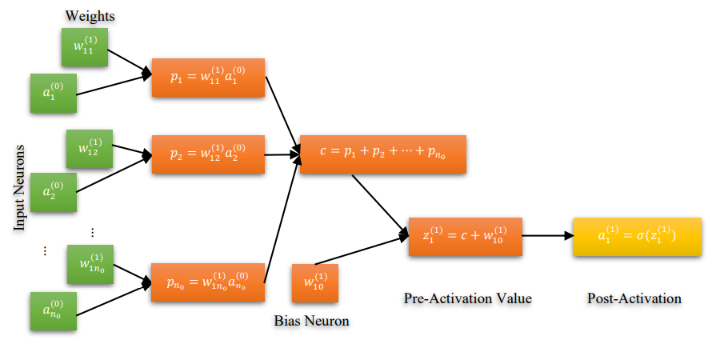
\includegraphics[width=\linewidth]{Images/04_Images/11.png}
    \caption{Đồ thị tính toán cho một nơ-ron}
\end{figure}
\paragraph{Ví dụ: biểu diễn một hàm bằng đồ thị tính toán\\}
Xét hàm hai biến
\begin{equation}
    F(x, y) = x^2 (x + y).
\end{equation}
Thay vì biểu diễn toàn bộ hàm bằng một biểu thức duy nhất, ta phân rã quá trình tính toán thành các phép toán trung gian. Đặt:
\begin{equation}
    c = x^2, \qquad s = x + y.
\end{equation}
Khi đó,
\begin{equation}
    F = cs.
\end{equation}
Đồ thị tính toán tương ứng có thể được mô tả bởi chuỗi phụ thuộc
\begin{equation}
    x, y \longrightarrow
    \begin{cases}
        c = x^2, \\
        s = x + y,
    \end{cases}
    \longrightarrow F = cs.
\end{equation}
Với $x = 2$ và $y = 3$, quá trình tính toán lần lượt cho
\begin{equation}
    c = 2^2 = 4, \qquad s = 2 + 3 = 5, \qquad F = 4 \cdot 5 = 20.
\end{equation}
Kết quả này tương đương với việc tính trực tiếp
\begin{equation}
    F = x^2 (x + y) = 2^2 (2 + 3) = 20.
\end{equation}
\begin{figure}[H]
    \centering
    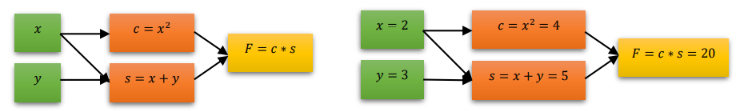
\includegraphics[width=\linewidth]{Images/04_Images/10.png}
    \caption{Đồ thị tính toán của hàm $F=x^2(x+y)$.}
\end{figure}
Ví dụ trên cho thấy đồ thị tính toán không thay đổi giá trị của hàm; thay vào đó, nó biểu diễn biểu thức dưới dạng một tập các phép tính cục bộ và các quan hệ phụ thuộc giữa chúng. Đây là đặc điểm có ý nghĩa quan trọng đối với việc tính đạo hàm bằng quy tắc chuỗi.
